%%%%%%%%%%%%%%%%%%%%%%%%%%%%%%%%%%%%%%%%%
% Beamer Presentation
% LaTeX Template
% Version 1.0 (10/11/12)
%
% This template has been downloaded from:
% http://www.LaTeXTemplates.com
%
% License:
% CC BY-NC-SA 3.0 (http://creativecommons.org/licenses/by-nc-sa/3.0/)
%
%%%%%%%%%%%%%%%%%%%%%%%%%%%%%%%%%%%%%%%%%

%----------------------------------------------------------------------------------------
%	PACKAGES AND THEMES
%----------------------------------------------------------------------------------------

\documentclass{beamer}

\usepackage{tikz}
\usetikzlibrary{arrows,automata,positioning}

\mode<presentation> {

% The Beamer class comes with a number of default slide themes
% which change the colors and layouts of slides. Below this is a list
% of all the themes, uncomment each in turn to see what they look like.

%\usetheme{default}
%\usetheme{AnnArbor}
%\usetheme{Antibes}
%\usetheme{Bergen}
%\usetheme{Berkeley}
%\usetheme{Berlin}
%\usetheme{Boadilla}
%\usetheme{CambridgeUS}
%\usetheme{Copenhagen}
%\usetheme{Darmstadt}
%\usetheme{Dresden}
%\usetheme{Frankfurt}
%\usetheme{Goettingen}
%\usetheme{Hannover}
%\usetheme{Ilmenau}
%\usetheme{JuanLesPins}
%\usetheme{Luebeck}
%\usetheme{Madrid}
%\usetheme{Malmoe}
%\usetheme{Marburg}
\usetheme{Montpellier}
%\usetheme{PaloAlto}
%\usetheme{Pittsburgh}
%\usetheme{Rochester}
%\usetheme{Singapore}
%\usetheme{Szeged}
%\usetheme{Warsaw}

% As well as themes, the Beamer class has a number of color themes
% for any slide theme. Uncomment each of these in turn to see how it
% changes the colors of your current slide theme.

%\usecolortheme{albatross}
%\usecolortheme{beaver}
%\usecolortheme{beetle}
%\usecolortheme{crane}
\usecolortheme{dolphin}
%\usecolortheme{dove}
%\usecolortheme{fly}
%\usecolortheme{lily}
%\usecolortheme{orchid}
%\usecolortheme{rose}
%\usecolortheme{seagull}
%\usecolortheme{seahorse}
%\usecolortheme{whale}
%\usecolortheme{wolverine}

%\setbeamertemplate{footline} % To remove the footer line in all slides uncomment this line
\setbeamertemplate{footline}[page number] % To replace the footer line in all slides with a simple slide count uncomment this line

\setbeamertemplate{navigation symbols}{} % To remove the navigation symbols from the bottom of all slides uncomment this line
}

\usepackage{graphicx} % Allows including images
\usepackage{booktabs} % Allows the use of \toprule, \midrule and \bottomrule in tables

%----------------------------------------------------------------------------------------
%	TITLE PAGE
%----------------------------------------------------------------------------------------

\title[INF210]{INF210 Overview} % The short title appears at the bottom of every slide, the full title is only on the title page

\author{Åsmund Kløvstad} % Your name
\institute[UiB] % Your institution as it will appear on the bottom of every slide, may be shorthand to save space
{
Universitetet i Bergen \\ % Your institution for the title page
}
\date{\today} % Date, can be changed to a custom date

\begin{document}

\begin{frame}
\titlepage % Print the title page as the first slide
\end{frame}

% \begin{frame}
% \frametitle{Overview} % Table of contents slide, comment this block out to remove it
% \tableofcontents % Throughout your presentation, if you choose to use \section{} and \subsection{} commands, these will automatically be printed on this slide as an overview of your presentation
% \end{frame}

%----------------------------------------------------------------------------------------
%	PRESENTATION SLIDES
%----------------------------------------------------------------------------------------

%------------------------------------------------
\section{State Transition Systems and Labeled Transition Systems} % Sections can be created in order to organize your presentation into discrete blocks, all sections and subsections are automatically printed in the table of contents as an overview of the talk
%------------------------------------------------

\begin{frame}
\frametitle{State Transition Systems}
\begin{itemize}
\item a tuple $(S, R)$
  \item $S = \{s_0,s_1...\}$
\item $R \subseteq S \times S$, often written $s \rightarrow s'$
  \item example: switch = $(\{s_0, s_1\}, \{ s_0 \times s_1, s_1 \times s_0\})$
\end{itemize}

\begin{figure}
  \centering
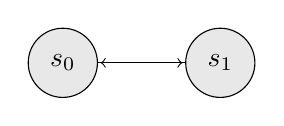
\begin{tikzpicture}[shorten >=1pt,node distance=2cm,on grid,auto] 
  \tikzstyle{every state}=[fill={rgb:black, 1;white,10}]

  \node[state] (s_0)                {$s_0$};
  \node[state] (s_1) [right of=s_0] {$s_1$};

  \path[->]
  (s_0) edge node {} (s_1)
  (s_1) edge node {} (s_0);
\end{tikzpicture}
  \end{figure}
\end{frame}

%------------------------------------------------

\begin{frame}
\frametitle{Important Properties of STSs}
\begin{itemize}
\item if a state has no rules going \textit{from} it, it is a \textbf{terminal
    state}.
\item if there is a sequence of steps from state $a$ to state $b$, $b$ is
  \textbf{reachable} from $a$. Write $R^*(a, b)$.
\item if $R$ is a function (in the set theory sense), then STS is \textbf{deterministic}.
\item we can make a non-deterministic STS deterministic with $(\mathcal{P}(S), R_\mathcal{P})$
\item if all paths eventually converge the STS is \textbf{confluent}.
\item switch is deterministic and confluent, and has no terminal states.
\end{itemize}
\end{frame}

%------------------------------------------------

\begin{frame}
\frametitle{Labeled Transition Systems}
\begin{block}{Syntax}
\begin{itemize}
\item extends STSs with labels
\item a 3-tuple $(S, L, R)$.
\item $R \subseteq S \times L \times S$, often written $s \xrightarrow{a} s'$
\end{itemize}
\end{block}
\begin{block}{Reachability}
\begin{itemize}
\item consider the STS $(S_L, R_L)$ with:
  \begin{itemize}
  \item $S_L = S \times L^*$
  \item $s \times a \cdot \mathbf{w} \rightarrow s' \times \mathbf{w} \in R_L$
    iff $s \xrightarrow{a} s' \in R$ 
   \end{itemize}
\item $s'$ is reachable from $s$ by $\mathbf{w}$ if $s' \times \lambda$ is
      reachable from $s \times \mathbf{w}$.
    \item write $s \times \mathbf{w} \vdash_{R}^* s' \times \lambda$
\end{itemize}
\end{block}
\end{frame}

%------------------------------------------------
\section{Languages, Grammars and Machines}
%------------------------------------------------

\begin{frame}
\frametitle{Languages}
\begin{itemize}
  \item language over alphabet: $L \subseteq \Sigma^*$
  \item ex. $\{a^nb^n \mid n \in \mathbb{N}\}$ over $\Sigma = \{a, b\}$
  \item deciding membership in a language
  \item classifying classes of languages
\end{itemize}
\begin{figure}
  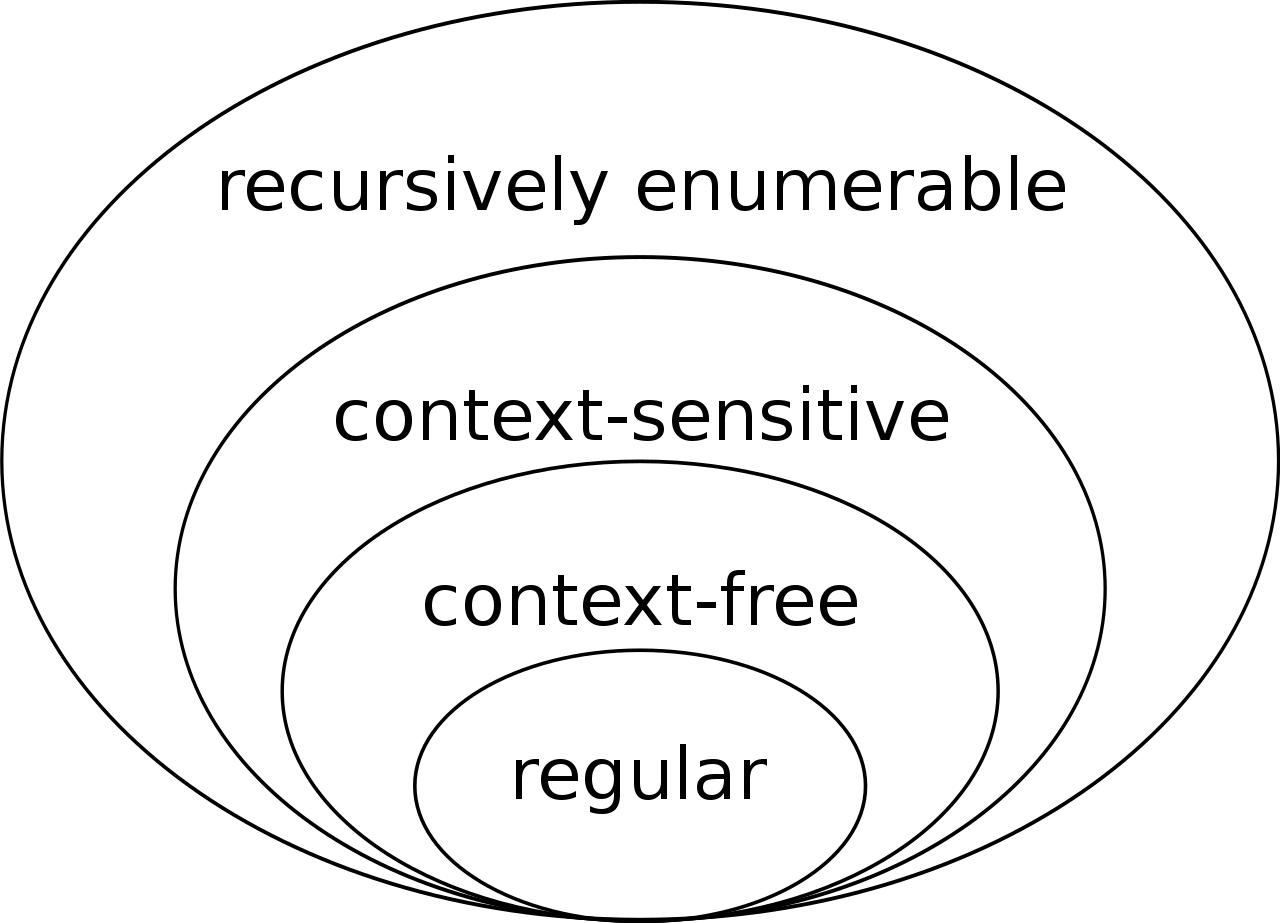
\includegraphics[height=0.4\textwidth]{Chomsky-hierarchy.png}
  \caption{from \url{https://en.wikipedia.org/wiki/Chomsky_hierarchy}}
\end{figure}
\end{frame}

%------------------------------------------------

\begin{frame}
\frametitle{Grammars}
\begin{itemize}
  \item $G = (\Sigma, N, S, \mathcal{R})$
  \item rules are $\mathbf{l} \Rightarrow \mathbf{r}$ with at least one
    non-terminal in $\mathbf{l}$
  \item \textbf{generates} a language over $\Sigma$
  \item $\mathbf{uav} \Rightarrow_G \mathbf{ubv}$ if $\mathbf{a}
    \Rightarrow \mathbf{b} \in \mathcal{R}$
  \item write $\mathbf{u} \Rightarrow_{G}^* \mathbf{v}$ for $\mathbf{u, v} \in
    (\Sigma \cup N)^*$ for ``\textbf{u} generates \textbf{v}''
  \item $L_G = \{\mathbf{w} \in \Sigma^* \mid S \Rightarrow_G^* \mathbf{w}\}$
  \item example: $G = (\{a\}, \{S\}, S, \{S \Rightarrow \lambda, S \Rightarrow
    Sa\})$ generates $a^*$
\end{itemize}
\end{frame}

%------------------------------------------------

\begin{frame}
\frametitle{Machines}
\begin{itemize}
  \item FA/FSM's, PDA's, TM's
  \item \textbf{accepts} input words
  \item $L_M = \{\text{words accepted by M}\}$
\end{itemize}
\end{frame}

%------------------------------------------------
\section{Finite Automata and Regular Languages}
%------------------------------------------------

\begin{frame}
\frametitle{Finite Automata}
\begin{itemize}
\item $M = (\Sigma, Q, q_0, \Upsilon, F)$
\item a finite LTS with initial and final states
\item the language accepted by $M$ is $L_M = \{\mathbf{w} \in \Sigma^* \; | \; q_0 \times
  \mathbf{w} \vdash_{\Upsilon}^* q_i \times \lambda \text{ and } q_i \in F\}$
\item deterministic/non-deterministic are equally powerful
\item example accepting $a^+b^+$
\begin{figure}
  \centering
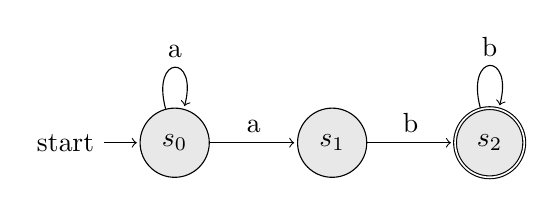
\begin{tikzpicture}[shorten >=1pt,node distance=2cm,on grid,auto] 
  \tikzstyle{every state}=[fill={rgb:black, 1;white,10}]

  \node[state, initial] (s_0)                {$s_0$};
  \node[state] (s_1) [right of=s_0] {$s_1$};
  \node[state, accepting] (s_2) [right of=s_1] {$s_2$};

  \path[->]
  (s_0) edge [loop above] node {a} (   )
        edge              node {a} (s_1)
  (s_1) edge              node {b} (s_2)
  (s_2) edge [loop above] node {b} (   );
\end{tikzpicture}
\caption{$M = (\{a, b\}, \{s_0, s_1, s_2\}, s_0, \{(s_0, a, s_0), (s_0, a, s_1),
  (s_1, b, s_2), (s_2, b, s_2)\}, \{s_2\})$}
\end{figure}
\end{itemize}
\end{frame}

%------------------------------------------------


\begin{frame}
  \frametitle{Regular Languages}
  \begin{itemize}
  \item \textbf{regular} languages are inductively defined by:
    \begin{itemize}
      \item $\emptyset, \{\lambda\}$ and $\{a\}$ are regular for $a \in \Sigma$
      \item if $L, L'$ regular, then $L \cup L', L \cdot L'$ and $L^*$ are
        regular
    \end{itemize}
   \item $\overline{L}$ and $L \cap L'$ are also regular
 \end{itemize}
\end{frame}

%------------------------------------------------

\begin{frame}
\frametitle{Kleene's Theorem}
\begin{theorem}
  a language is regular $\iff$ it is accepted by a finite automata
\end{theorem}
\begin{block}{$\Rightarrow$}
Construct FAs for the empty language, $\{\lambda\}$ and singleton
languages. Then construct FAs for union, concatenation, and Kleene star.
\end{block}

\begin{block}{$\Leftarrow$}
Define $R(i, k, j) = \{\mathbf{w} \; | \; q_j \text{ is reachable from } q_i
\text{ by } \mathbf{w}
\text{ without visiting } q_m \text{ with } m \geq k\}$\\

Then show $R(i, k+1, j) = R(i, k, j) \cup R(i, k, k) \cdot R(k, k, k)^* \cdot
R(k, k, j)$
\end{block}
\end{frame}

%------------------------------------------------

\begin{frame}
\frametitle{Pumping Lemma}
\begin{itemize}
  \item if $L$ is regular then there exists some $n > 0$ s.t for any $\mathbf{w}
    \in L$ longer than $n$, $\mathbf{w} = \mathbf{xyz}$ with $\lvert \mathbf{y} \rvert
    \geq 1$ and $\lvert \mathbf{xy} \leq n \rvert$
    Then $\mathbf{xy^kz} \in L$ for all $k \geq 0$
  \item makes sense because some state must be visited twice
  \item very useful for showing a language is \textbf{not} regular
\end{itemize}
\end{frame}

%------------------------------------------------

\subsection{Syntactic Monoids and Transformation Monoids}
\begin{frame}
\frametitle{Syntactic Monoid of a Language}
\begin{itemize}
  \item given a language $L$ over $\Sigma$
  \item $LR(\mathbf{w}) = \{\mathbf{x} \times \mathbf{y} \mid \mathbf{xwy} \in L\}$
  \item $\mathbf{u} \approx \mathbf{v} := LR(\mathbf{u}) = LR(\mathbf{v})$
  \item this is left-right invariant, so $[\mathbf{u}]_\approx
    \cdot [\mathbf{v}]_\approx := [\mathbf{uv}]_\approx$ is well defined
  \item $(\Sigma^*_{/ \approx}, \cdot, [\lambda]_\approx)$ is the
    \textbf{syntactic monoid} of $L$.
\end{itemize}
\end{frame}

%------------------------------------------------

\begin{frame}
\frametitle{Transformation Monoid of a FA}
\begin{itemize}
\item given $M = (\Sigma, Q, q_0, \Upsilon, F)$
\item each $a \in \Sigma$ induces a function $\overline{a} : Q \rightarrow Q$
    by $q \mapsto \Upsilon(q, a)$
\item with $\overline{\lambda} = id_{Q}$ and $\overline{\mathbf{w}a} =
        \overline{\mathbf{w}} \circ \overline{a}$ this extends to words
\item $\overline{\mathbf{vw}} = \overline{\mathbf{v}} \circ
  \overline{\mathbf{w}}$, so $\overline{} : \Sigma^* \rightarrow (Q \rightarrow
  Q)$ is a (monoid) homomorphism
\item call the image $\overline{\Sigma^*} \subseteq (Q \rightarrow Q)$ the
  \textbf{transformation monoid} of $M$
\item the syntactic monoid of $L$ $\cong$ the transformation monoid of $M_L$
  (intrinsic/minimal FA)
\end{itemize}
\end{frame}

\begin{frame}
\frametitle{Regular Grammars}
  \begin{itemize}
  \item rules are either $A \Rightarrow B$,
    $A \Rightarrow aB$ or $A \Rightarrow \lambda$ for $A, B \in N, a \in \Sigma$
  \item generate regular languages
  \item let FA $M = (\Sigma, N \cup \{f\}, S, \Upsilon, \{A \in N \mid A
    \Rightarrow \lambda \in \mathcal{R}\})$ with $\Upsilon$:
    \begin{itemize}
      \item $A \xrightarrow{a} B$ for $A \Rightarrow aB \in \mathcal{R}$
      \item $A \xrightarrow{a} f$ for $A \Rightarrow a \in \mathcal{R}$
    \end{itemize}
  \item then $L_M = L_G$
  \end{itemize}
\end{frame}

%------------------------------------------------
\section{Pushdown Automata and Context Free Languages}
%------------------------------------------------

%------------------------------------------------

\begin{frame}
\frametitle{Pushdown Automata}
\begin{itemize}
\item finite automaton with a stack:
  \begin{itemize}
  \item $\Sigma$: an alphabet
  \item $\Gamma$: a stack alphabet
  \item $Q$: a finite set of states
  \item $q_0 \in Q$: an initial state
  \item $\Delta \subseteq Q \times (\Sigma_\lambda \times \Gamma_\lambda \times
    \Gamma_\lambda) \times Q$: a transition relation
  \item $F \subseteq Q$: a set of final states
  \end{itemize}
\item accepts in final state with empty stack
  \item example:
\end{itemize}
\begin{figure}
  \centering
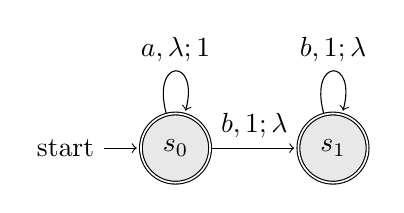
\begin{tikzpicture}[shorten >=1pt,node distance=2cm,on grid,auto] 
  \tikzstyle{every state}=[fill={rgb:black, 1;white,10}]

  \node[state, initial, accepting] (s_0)       {$s_0$};
  \node[state, accepting] (s_1) [right of=s_0] {$s_1$};

  \path[->]
  (s_0) edge node {$b, 1; \lambda$} (s_1)
        edge [loop above] node {$a, \lambda; 1$} ()
  (s_1) edge [loop above] node {$b, 1; \lambda$} ();
\end{tikzpicture}
  \end{figure}
\end{frame}

%------------------------------------------------

\begin{frame}
\frametitle{Context Free Grammars}
\begin{itemize}
\item left hand side is a single non-terminal
\item generate a superset of regular languages
\item call this class \textbf{context free} languages
\item ex. $S \Rightarrow \lambda, S \Rightarrow aSb$ generates $a^nb^n$
\end{itemize}
\end{frame}

%------------------------------------------------

\begin{frame}
\frametitle{Context Free Languages}
\begin{theorem}{}
  a language is context free $\iff$ it is accepted by a pushdown automata
\end{theorem}
\begin{block}{$\Leftarrow$}
  Given PDA $M = (\Sigma, \Gamma, \{s_0\}, s_0, !, \Delta)$ construct $G' =
  (\Sigma, \Gamma, !, \mathcal{R})$ with $\mathcal{R}$:
  \begin{itemize}
  \item $A \Rightarrow a\mathbf{W}$ for each $(a, A; \mathbf{W}) \in \Delta$
    \item $A \Rightarrow \mathbf{W}$ for each $(\lambda, A; \mathbf{W}) \in \Delta$
   \end{itemize}
  note: empty stack acceptance, start with ! on stack, allow pushing words
\end{block}
\end{frame}
%------------------------------------------------

\begin{frame}
\frametitle{Context Free Languages}
\begin{theorem}{}
  a language is context free $\iff$ it is accepted by a pushdown automata
\end{theorem}
\begin{block}{$\Rightarrow$}
  Given CFG $G = (\Sigma, N, S, \mathcal{R})$ construct:
\begin{figure}
  \centering
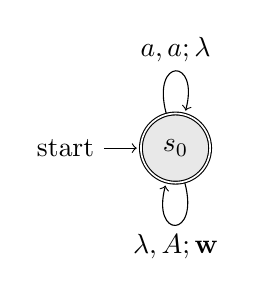
\begin{tikzpicture}[shorten >=1pt,node distance=2cm,on grid,auto] 
  \tikzstyle{every state}=[fill={rgb:black, 1;white,10}]

  \node[state, initial, accepting] (s_0)       {$s_0$};

  \path[->]
  (s_0) edge [loop above] node {$a, a; \lambda$} ()
        edge [loop below] node {$\lambda, A; \mathbf{w}$} ();
\end{tikzpicture}
  \end{figure}
  for each $a \in \Sigma$ and $A \Rightarrow \mathbf{w} \in \mathcal{R}$\\
\end{block}
\end{frame}

%------------------------------------------------

\begin{frame}
\frametitle{Parsing}
\begin{itemize}
  \item given a $\mathbf{w} \in \Sigma^*$, identify syntactic structure
  \item top-down: attempt to generate $\mathbf{w}$ from $S$ (PDA)
  \item bottom-up: split into subwords and find rules to generate them
\end{itemize}
\begin{figure}
  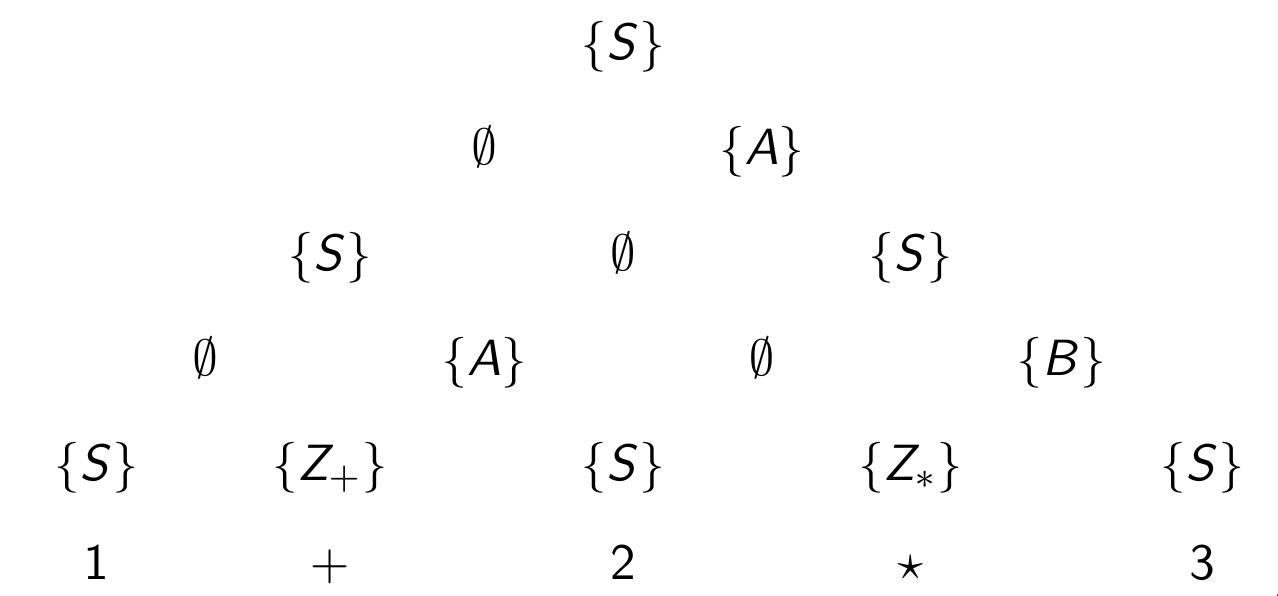
\includegraphics[width=0.8\textwidth]{Parse-tree.png}
  \caption{from \texttt{Parsing.pdf}}
\end{figure}
\end{frame}

%------------------------------------------------

\begin{frame}
\frametitle{Pumping Lemma for CFLs}
\begin{itemize}
  \item given CFG $G = (\Sigma, N, S, \mathcal{R})$
  \item any $\mathbf{s} \in L_G$ longer than $2^{\lvert N \rvert - 1}$ can be
    written as $\mathbf{s} = \mathbf{uvwxy}$ with $\lvert \mathbf{vx} \rvert
    \geq 1$ s.t
    $\mathbf{uv}^n\mathbf{wx}^n\mathbf{y} \in L_G$ for all $n \in \mathbb{N}$
\end{itemize}
\begin{figure}
  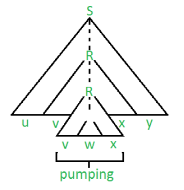
\includegraphics[width=0.3\textwidth]{CFL-pumping-lemma.png}
  \caption{from \url{https://www.geeksforgeeks.org/pumping-lemma-in-theory-of-computation/}}
  \end{figure}
\end{frame}


%------------------------------------------------
\section{Turing Machines}
%------------------------------------------------

\begin{frame}
\frametitle{Turing Machine}
\begin{itemize}
\item $M = (Q, \Sigma, q_0, \delta, H)$ with:
  \begin{itemize}
  \item $Q$: a finite set of states
  \item $\Sigma$: a finite alphabet which includes the blank symbol \#
  \item $q_0 \in Q$: a starting state
  \item $\delta: (Q \setminus H) \times \Sigma \rightarrow Q \times \Sigma
    \times \{-1, 0, 1\}$: a (possibly partial) transition function
  \item $H = \{h_0, h_1\}$: a rejecting and an accepting halting state
  \end{itemize}
\item a head with state reading an infinite tape
\item accepts a word \textbf{w} iff it halts in $h_1$ when started with \textbf{w} on the tape
\item \textbf{decides} a language only if $h_0$ is reached for $\mathbf{w} \not\in L$
\end{itemize}
\end{frame}

%------------------------------------------------

\begin{frame}
\frametitle{Phrase-Structure Grammars}
\begin{itemize}
\item grammars with rules $\mathbf{u} \Rightarrow \mathbf{w}$ s.t \textbf{u} has
  at least one non-terminal
\item as powerful as Turing Machines
\end{itemize}
\begin{block}{}
Create a PSG which work like:
 \begin{enumerate}
 \item generate $\{\mathbf{w}!q_0H\mathbf{w}!\}$
 \item maintain \textbf{w}! [tape] [state] H [tape] !
 \item when state is $h_1$, remove everything between !'s (and then the !'s)
 \end{enumerate}
\end{block}
\end{frame}

%------------------------------------------------

\begin{frame}
\frametitle{Halting Problem}
\begin{theorem}
  Standardize and enumerate all Turing Machines $\{T_i\}$. Let $L = \{1^i01^j
  \mid T_i \text{ halts on input } 1^j\}$\\
  Then there is no Turing Machine which decides $L$
\end{theorem}
\begin{itemize}
\item assume $M$ decides $L$
\item construct $M'$ s.t it acts on input $1^i$:
  \begin{enumerate}
  \item change tape to $1^i01^i$
  \item move to first cell
  \item emulate $M$ on the tape
  \item if $M$ accepts, loop infinitely. if $M$ rejects, reject
  \end{enumerate}
\item enumerate $M' = T_k$ and run $M$ with $1^k01^k$ as input 
\item if $M$ accepts, then $M'$ halts with $1^k$ as input, so $M$ must reject by 4.
\item if $M$ rejects, then $M'$ loops forever, so $M$ must accept by 4.
\end{itemize}
\end{frame}

%------------------------------------------------

\section{Splicing Languages}
\begin{frame}
\frametitle{Splicing Languages}
\begin{itemize}
  \item abstracts DNA as a word over $\Sigma = \{a, c, g, t\}$
  \item splicing rules: $(\mathbf{u, u', v, v'}) \in (\Sigma^*)^4$
  \item splicing action: split between \textbf{u,u'} and \textbf{v,v'}.
    Recombine \textbf{uv'}
  \item splicing system: $(\Sigma, R, l)$ with an alphabet, set of rules,
    finite initial language
  \item language generated by system: smallest closed language
  \item L is a \textbf{splicing language} if it is generated by some splicing system
  \item given a regular language and a set of splicing rules, we can check if
    the language respects the rules
\end{itemize}
\end{frame}

%------------------------------------------------

% \section{Appendix}
% \begin{frame}
% \frametitle{Other stuff that might be nice}
% \begin{itemize}
% \item diagrams for FA's in Kleene's theorem
% \item diagram from R(i, k, j) for Kleene's theorem
% \item procedure for making deterministic STS/LTS/FA
% \item getting rid of epsilon steps
% \item what exactly is the intrinsic FA of a language
% \item regular grammar <-> FSM correspondence
% \item PSG <-> TM correspondence
% \end{itemize}
% \end{frame}
\end{document} 